
\documentclass[11pt,a4paper]{article}

\usepackage[margin=2.2cm]{geometry}
\usepackage{amsmath,amssymb,mathtools}
\usepackage{booktabs}
\usepackage{enumitem}
\usepackage{microtype}
\usepackage{hyperref}
\usepackage{xcolor}

\usepackage{tikz}
\usetikzlibrary{arrows.meta,positioning,fit,calc,shapes.multipart,shapes.geometric}

\usepackage{pgfplots}
\pgfplotsset{compat=1.18}

\usepackage[ruled,vlined]{algorithm2e}

\title{\vspace{-1.2em}MOSinLine --- Integrated Optimization--Simulation Workflow (Final Integration Note)}
\author{Kailin Yang \and Johannes Kager \and  \textit{(project team)}}
\date{\vspace{-0.8em}\today}

\begin{document}
\maketitle

\noindent\textbf{Context.}
MOSinLine combines strategic network design, tactical delivery pattern planning, and discrete-event simulation
into an integrated workflow to support sustainable grocery retail logistics under demand uncertainty.
This short report documents the final integration step: a single algorithm that executes
\emph{(i)} robust warehouse location/sizing and store assignment (ASBP / robust LRP),
\emph{(ii)} delivery pattern planning (PATT),
and \emph{(iii)} network evaluation in AnyLogic (SIM),
and iteratively updates parameters (weights, scenario emphasis, demand slack) based on simulation feedback.
(See project outline for the overarching motivation and AP structure.)\par

\vspace{0.8em}
\noindent\textbf{Notation (high level).}
Let $J$ be the set of stores, $I$ candidate warehouse sites, $D$ days in a week, $P$ product categories, $S$ demand scenarios.
We use $\lambda\in[0,1]$ as a weight between economic and environmental objectives.

\section{Three building blocks and interfaces}

Figure~\ref{fig:threeblocks} summarizes inputs/outputs and the planned data flow between the three modules.

\begin{figure}[t]
\centering
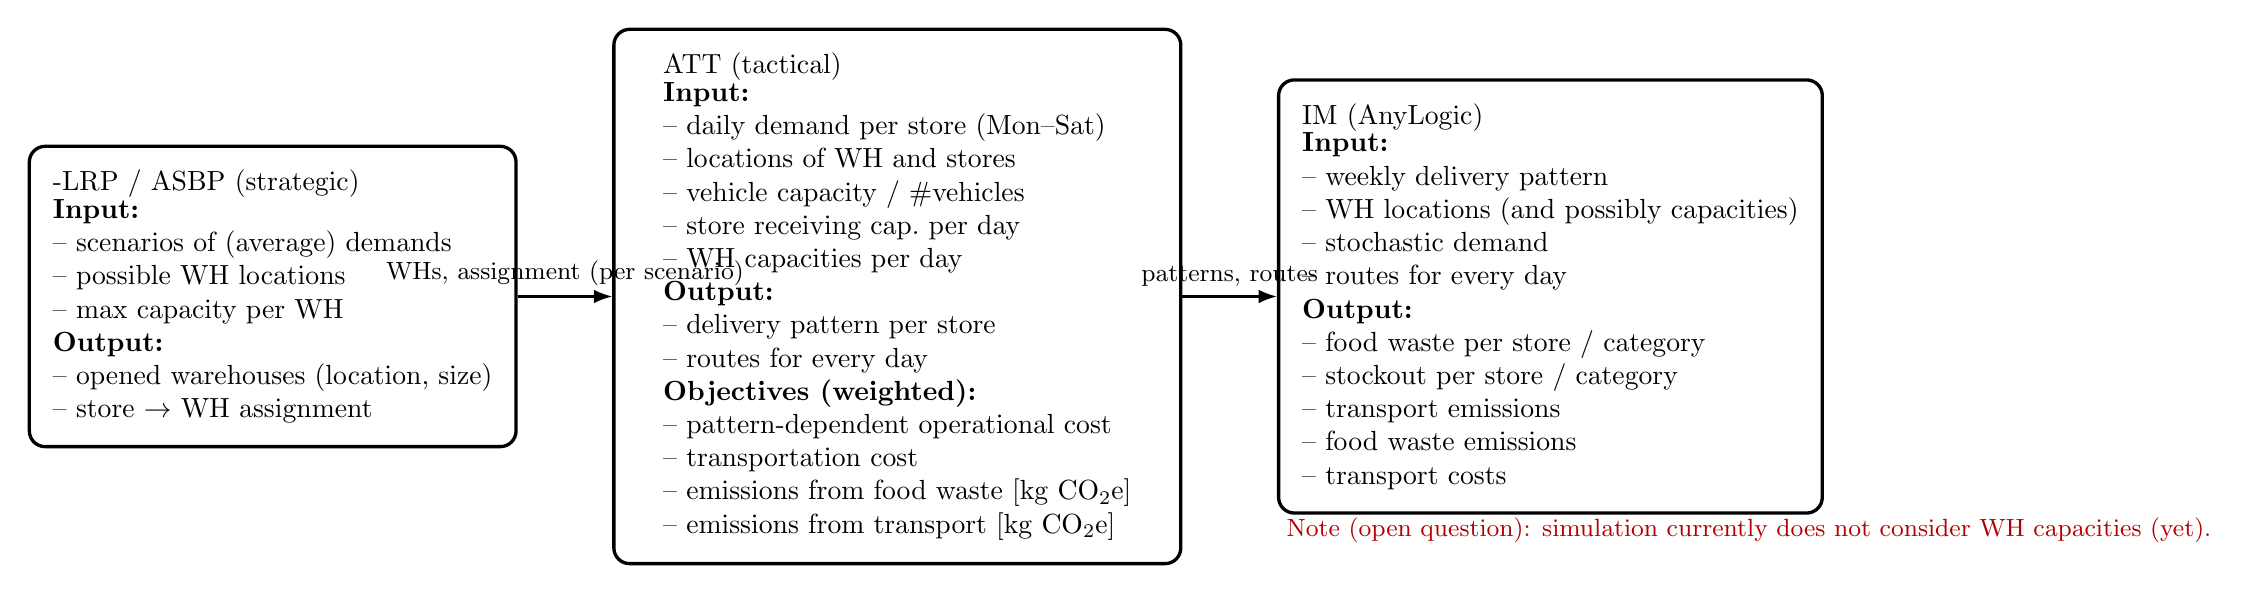
\begin{tikzpicture}[
  box/.style={draw, rounded corners=2mm, very thick, inner sep=3mm, align=left},
  title/.style={font=\bfseries},
  arr/.style={-Latex, thick},
  note/.style={font=\small, align=left}
]
\node[box] (rlrp) {
  {\title R-LRP / ASBP (strategic)}\\[-0.2em]
  \textbf{Input:}\\
  -- scenarios of (average) demands\\
  -- possible WH locations\\
  -- max capacity per WH\\
  \textbf{Output:}\\
  -- opened warehouses (location, size)\\
  -- store $\rightarrow$ WH assignment
};

\node[box, right=1.2cm of rlrp, minimum width=7.2cm] (patt) {
  {\title PATT (tactical)}\\[-0.2em]
  \textbf{Input:}\\
  -- daily demand per store (Mon--Sat)\\
  -- locations of WH and stores\\
  -- vehicle capacity / \#vehicles\\
  -- store receiving cap.\ per day\\
  -- WH capacities per day\\
  \textbf{Output:}\\
  -- delivery pattern per store\\
  -- routes for every day\\
  \textbf{Objectives (weighted):}\\
  -- pattern-dependent operational cost\\
  -- transportation cost\\
  -- emissions from food waste [kg CO$_2$e]\\
  -- emissions from transport [kg CO$_2$e]
};

\node[box, right=1.2cm of patt] (sim) {
  {\title SIM (AnyLogic)}\\[-0.2em]
  \textbf{Input:}\\
  -- weekly delivery pattern\\
  -- WH locations (and possibly capacities)\\
  -- stochastic demand\\
  -- routes for every day\\
  \textbf{Output:}\\
  -- food waste per store / category\\
  -- stockout per store / category\\
  -- transport emissions\\
  -- food waste emissions\\
  -- transport costs
};

\draw[arr] (rlrp.east) -- node[above, note]{WHs, assignment (per scenario)} (patt.west);
\draw[arr] (patt.east) -- node[above, note]{patterns, routes} (sim.west);

\node[note, below=0.2cm of sim.south west, anchor=west, text=red!70!black]
{Note (open question): simulation currently does not consider WH capacities (yet).};

\end{tikzpicture}
\caption{Three components and their interfaces. Extracted from the integration sketch.}
\label{fig:threeblocks}
\end{figure}

\section{Demand representations and aggregation between modules}

The three modules operate on different demand resolutions:
\begin{itemize}[leftmargin=1.4em]
\item \textbf{R-LRP:} one nonnegative real number per store and scenario (weekly or average).
\item \textbf{PATT:} daily demand per store and day-of-week.
\item \textbf{SIM:} stochastic daily demand per store, day-of-week, and product category (e.g., Poisson with given mean),
with repeated weekly replications.
\end{itemize}

\subsection{From SIM to PATT and R-LRP}

Let $\bar\beta^{s}_{jpd}$ denote the \emph{mean} daily demand (e.g., kg) for store $j\in J$,
product category $p\in P$, weekday $d\in D$, and scenario $s\in S$.
A simulation run draws realizations around these means and evaluates KPIs.

\paragraph{Aggregation to PATT (sum over categories).}
\begin{equation}
  \beta^{s}_{jd} \;=\; \sum_{p\in P} \bar\beta^{s}_{jpd}
  \qquad (j\in J,\; d\in D,\; s\in S).
  \label{eq:sim-to-patt}
\end{equation}

\paragraph{Aggregation to R-LRP (collapse day-of-week).}
Several options are plausible, depending on how conservative the strategic model should be:
\begin{align}
  \beta^{s}_{j} &= \frac{1}{|D|}\sum_{d\in D} \beta^{s}_{jd} 
  &&\text{(average day)} \label{eq:patt-to-rlrp-avg}\\
  \beta^{s}_{j} &= \max_{d\in D} \beta^{s}_{jd} 
  &&\text{(peak day)} \label{eq:patt-to-rlrp-max}\\
  \beta^{s}_{j} &= \text{2nd/3rd value of }\text{sort-desc}\bigl(\beta^{s}_{jd}:d\in D\bigr)
  &&\text{(robust but less extreme)} \label{eq:patt-to-rlrp-quant}
\end{align}
The ``right'' choice can be scenario-dependent and may reflect seasonality over the year.

\begin{figure}[t]
\centering
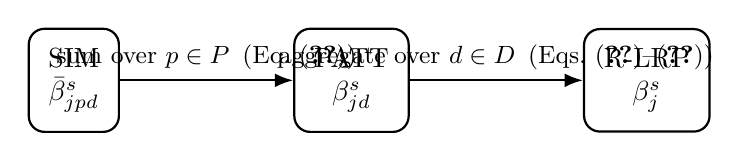
\begin{tikzpicture}[
  n/.style={draw, rounded corners=2mm, thick, inner sep=2.5mm, align=center},
  arr/.style={-Latex, thick},
  lab/.style={font=\small}
]
\node[n] (sim) {SIM\\ $\bar\beta^{s}_{jpd}$};
\node[n, right=2.2cm of sim] (patt) {PATT\\ $\beta^{s}_{jd}$};
\node[n, right=2.2cm of patt] (rlrp) {R-LRP\\ $\beta^{s}_{j}$};

\draw[arr] (sim) -- node[above, lab]{sum over $p\in P$ \,(Eq.~\eqref{eq:sim-to-patt})} (patt);
\draw[arr] (patt) -- node[above, lab]{aggregate over $d\in D$ \,(Eqs.~\eqref{eq:patt-to-rlrp-avg}--\eqref{eq:patt-to-rlrp-quant})} (rlrp);
\end{tikzpicture}
\caption{Demand aggregation chain used for interfacing SIM, PATT, and R-LRP.}
\label{fig:demandchain}
\end{figure}

\section{Objective alignment and KPI set}

\subsection{KPI set used for simulation feedback}

We track a small set of KPIs per replication $r$ and scenario $s$, e.g.
\[
\text{KPI} \in \{\text{OC}, \text{TC}, \text{FWE}, \text{TE}\},
\]
where OC = operational costs, TC = transport costs, FWE = food-waste emissions, TE = transport emissions.
A simple acceptance rule from the sketch is:
\begin{itemize}[leftmargin=1.4em]
\item No KPI has \emph{mean over replications and scenarios} exceeding a threshold.
\item No KPI has \emph{worst-case (over scenarios) mean} exceeding a threshold.
\item Ultimately, acceptability is determined by the decision maker.
\end{itemize}

\subsection{Common weighting parameter $\lambda$}

Both optimization modules use a common weighting parameter $\lambda\in[0,1]$ to interpolate between
economic costs and CO$_2$e-related terms. Conceptually:
\begin{equation}
  \min\;\; (1-\lambda)\cdot \text{Cost} \;+\; \lambda\cdot \text{CO$_2$e}.
  \label{eq:lambda-weight}
\end{equation}

\begin{figure}[t]
\centering
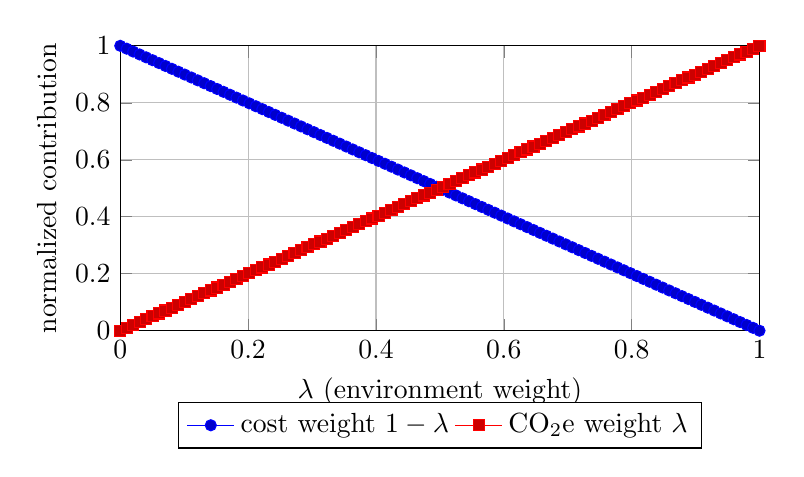
\begin{tikzpicture}
\begin{axis}[
  width=0.80\linewidth,
  height=5.2cm,
  xlabel={$\lambda$ (environment weight)},
  ylabel={normalized contribution},
  xmin=0, xmax=1,
  ymin=0, ymax=1,
  legend style={at={(0.5,-0.25)},anchor=north,legend columns=2},
  grid=both
]
% schematic only
\addplot+[domain=0:1, samples=100] {1-x};
\addlegendentry{cost weight $1-\lambda$}
\addplot+[domain=0:1, samples=100] {x};
\addlegendentry{CO$_2$e weight $\lambda$}
\end{axis}
\end{tikzpicture}
\caption{Schematic visualization of the shared weighting parameter $\lambda$.}
\label{fig:lambda}
\end{figure}

\section{Strategic model: (robust) capacitated location--routing objective sketch}

For the strategic robust location--routing model (RCLRP/R-LRP), the notes propose a two-stage objective of the form
\begin{equation}
  \min_{x} \; f(x) \;+\; \max_{s\in S} \min_{y^s} g^s(x,y^s)\cdot \delta^s,
  \label{eq:two-stage-sketch}
\end{equation}
where $\delta^s$ can emphasize particular scenarios (e.g., set $\delta^{1}=1.1$ and $\delta^{s}=1$ for $s\neq 1$).

A more concrete decomposition uses first-stage warehouse opening variables $w_i^0\in\{0,1\}$ and sizes $a_i^0\in\mathbb{Z}_+$:
\begin{equation}
  f(w^0,a^0) \;=\; \sum_{i\in I} e_i\, w_i^0 \;+\; \sum_{i\in I} d_i\, a_i^0,
  \label{eq:rlrp-firststage}
\end{equation}
plus second-stage ``recovery'' terms (open/expand warehouses and route under scenario $s$):
\begin{align}
  g^s(\cdot) \;=\;
  &\sum_{i\in I} e'_i\,(w_i^s-w_i^0)
  \;+\; \sum_{i\in I} d'_i\,(a_i^s-a_i^0) \nonumber\\
  &+ \sum_{(v_1,v_2)\in E} c_{v_1,v_2}\, r^s_{v_1,v_2}
  \;+\; \sum_{(v_1,v_2)\in E} \alpha_{v_1,v_2}\, r^s_{v_1,v_2} \nonumber\\
  &+ \sum_{(v_1,v_2)\in E} \gamma_{v_1,v_2}\, t^s_{v_1,v_2}
  \;+\; \sum_{i\in I,\,j\in J} F\, r^s_{i,j}.
  \label{eq:rlrp-secondstage}
\end{align}
Here $r^s_{v_1,v_2}$ indicates arc usage and $t^s_{v_1,v_2}$ transported load, while $c$ is traversal cost,
$\alpha$ is CO$_2$e of an empty vehicle on the arc, $\gamma$ is marginal CO$_2$e per unit load, and $F$ is a fixed cost per used vehicle.

\paragraph{Parameter heuristics noted during integration.}
\begin{center}
\begin{tabular}{@{}ll@{}}
\toprule
Item & Sketch values / notes \\
\midrule
Opening vs sizing costs & $e_i \approx 10\, d_i$; $d_i\in[1.25,3.5]$ \\
Capacity & $A_i \in [60,120]$ (max WH capacity) \\
Recovery multipliers & $e'_i = 1.5\,e_i$, $d'_i = 1.5\,d_i$ \\
Distances & $c_{ij}\in[0,82]$ km (avg $\approx 36$ km) \\
Vehicle cap. & $20$ \\
Demand noise & $\varepsilon \in [0,5]$ (interpreted as $\approx 20\%$) \\
CO$_2$ factors & $\alpha_{ij} = 0.0635\cdot 8.706\cdot c_{ij}$,\quad
$\gamma_{ij} = 0.001004\cdot 8.706\cdot c_{ij}$ \\
Fixed vehicle cost & $F=100$ (note: set $F=0$ in PATT alignment) \\
\bottomrule
\end{tabular}
\end{center}

\section{Tactical model: delivery pattern planning (PATT)}

For delivery pattern planning, the provided model minimizes a weighted sum of economic and environmental terms:
\begin{align}
  \min Z \;=\; &(1-\lambda)\Bigg[
  \sum_{f\in F\setminus\{0\}}\sum_{r\in R} c^{\text{PAT}}_{f,r}\, x_{f,r}
  \;+\;\sum_{k\in K}\sum_{t\in T}\sum_{i\in F}\sum_{j\in F\setminus\{i\}}
  c^{\text{TR}}_{i,j}\, v_{k,t,i,j}
  \Bigg] \nonumber\\
  &+\lambda\Bigg[
  \sum_{f\in F\setminus\{0\}}\sum_{r\in R} e^{\text{FW}}_{f,r}\, x_{f,r}
  \;+\;\sum_{k\in K}\sum_{t\in T}\sum_{i\in F}\sum_{j\in F\setminus\{i\}}
  \bigl(e^{\text{P0}}_{i,j}\, v_{k,t,i,j} + e^{\text{P1}}_{i,j}\, f_{k,t,i,j}\bigr)
  \Bigg].
  \label{eq:patt-obj}
\end{align}
Constraints include: pattern selection, pattern--day linkage, daily quantity limits, store receiving capacity,
depot departure/return, flow conservation, MTZ subtour elimination, visit requirement, delivered quantities,
load balance, arc flow capacity, and vehicle usage.

\paragraph{Coefficient alignment (integration note).}
The sketch notes the mapping
$c^{\text{TR}}\leftrightarrow c$, $e^{\text{P0}}\leftrightarrow \alpha$, $e^{\text{P1}}\leftrightarrow \gamma$,
and using $F=0$ in the PATT model. Additionally, the strategic model contains parameters (e.g., $e$ and $d$)
that do not appear in the PATT model and thus require separate calibration (e.g., warehouse costs per week).

\section{Integrated algorithm (single workflow)}

Figure~\ref{fig:loop} shows the core integration loop:
solve R-LRP per scenario/setting, feed resulting warehouses and assignments into PATT,
evaluate in SIM over replications/weeks, then update weights (and optionally demand slack or scenario weights)
until the solution is ``good enough''.

\begin{figure}[t]
\centering
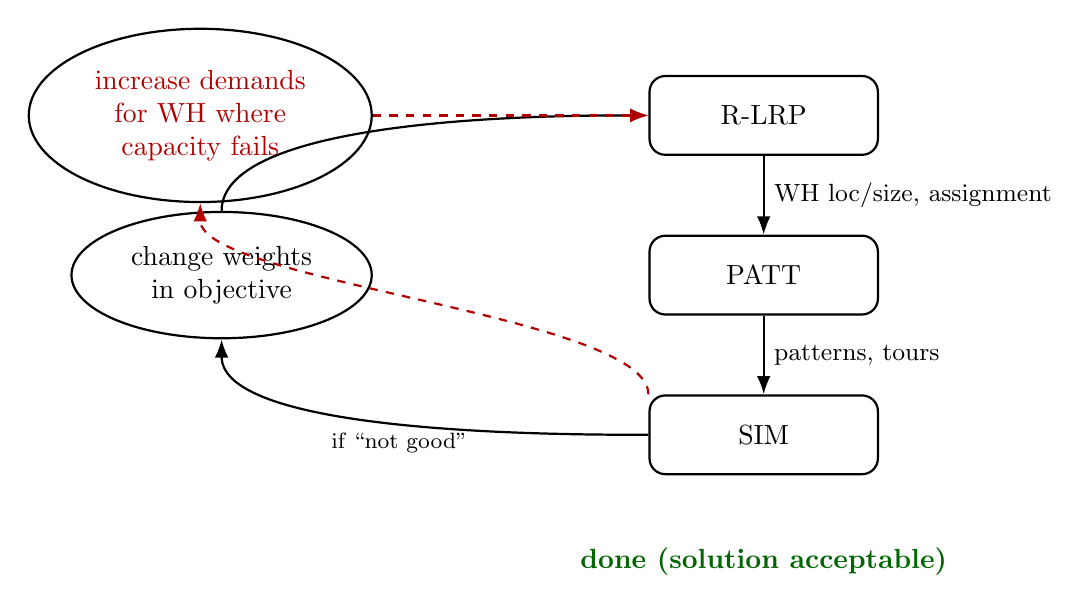
\begin{tikzpicture}[
  b/.style={draw, rounded corners=2mm, thick, minimum width=2.9cm, minimum height=1.0cm, align=center},
  a/.style={-Latex, thick},
  c/.style={draw, ellipse, thick, align=center, inner sep=2mm}
]
\node[b] (A) {R-LRP};
\node[b, below=1.0cm of A] (B) {PATT};
\node[b, below=1.0cm of B] (C) {SIM};
\node[c, left=3.5cm of B] (W) {change weights\\in objective};
\node[c, left=3.5cm of A, text=red!70!black] (S) {increase demands\\for WH where\\capacity fails};

\draw[a] (A) -- node[right,font=\small]{WH loc/size, assignment} (B);
\draw[a] (B) -- node[right,font=\small]{patterns, tours} (C);
\draw[a] (C.west) .. controls +(left:1.2cm) and +(down:1.2cm) .. node[below,font=\small]{\footnotesize if ``not good''} (W.south);
\draw[a] (W.north) .. controls +(up:1.2cm) and +(left:1.2cm) .. (A.west);
\draw[a, dashed, color=red!70!black] (C.north west) .. controls +(up:1.0cm) and +(down:1.0cm) .. (S.south);
\draw[a, dashed, color=red!70!black] (S.east) -- (A.west);

\node[below=0.8cm of C, font=\bfseries, text=green!40!black] {done (solution acceptable)};
\end{tikzpicture}
\caption{Iterative integration loop (schematic).}
\label{fig:loop}
\end{figure}

\begin{algorithm}[t]
\DontPrintSemicolon
\SetKwInOut{Input}{Input}\SetKwInOut{Output}{Output}
\Input{Scenario set $S$ with mean demands $\bar\beta^s_{jpd}$; candidate WH sites $I$; stores $J$; initial weights $\lambda$ and scenario weights $\delta$; simulation settings (\#weeks, \#replications).}
\Output{Integrated solution: WH locations/sizes, assignments, delivery patterns, routes; evaluated KPIs.}

\BlankLine
Initialize $\lambda\gets\lambda_0$ and $\delta^s\gets 1$ for all $s\in S$\;
\While{not accepted}{
  \tcp{(1) Demand preprocessing}
  Aggregate $\bar\beta^s_{jpd}$ to PATT demands $\beta^s_{jd}$ via~\eqref{eq:sim-to-patt} and to R-LRP demands $\beta^s_j$ via~\eqref{eq:patt-to-rlrp-avg}--\eqref{eq:patt-to-rlrp-quant}\;

  \tcp{(2) Strategic optimization (ASBP / robust LRP)}
  Solve R-LRP for each scenario $s$ (or for an aggregated robust instance) using weights $(\lambda,\delta)$\;
  Obtain WH decisions (location/size) and store assignments (possibly scenario-dependent)\;

  \tcp{(3) Tactical optimization (delivery patterns)}
  For each scenario $s$ (and resulting assignment), solve PATT with the same $\lambda$ to obtain store patterns and daily routes\;

  \tcp{(4) Simulation evaluation}
  Run AnyLogic SIM for each $s$ over multiple replications/weeks; collect KPI samples $\text{KPI}_{r,s}$\;

  \tcp{(5) Feedback / parameter update}
  If KPI thresholds violated: update $\lambda$ (and optionally scenario weights $\delta$);\\
  optionally increase (some) demands or WH sizes if WH capacity is a binding issue\;
}
\caption{Single integrated workflow (final integration step).}
\label{alg:integrated}
\end{algorithm}

\section{Open integration issues and practical notes}

\begin{itemize}[leftmargin=1.4em]
\item \textbf{Warehouse capacity in simulation:} decide whether SIM enforces WH throughput/capacity constraints
and how this feeds back (capacity violations $\Rightarrow$ demand slack or strategic resizing).
\item \textbf{Warehouse cost scaling:} consider expressing warehouse opening/sizing costs per week to align with
weekly PATT/SIM evaluation; calibrate using a reference facility (e.g., Straubing) by relating area/throughput to cost.
\item \textbf{Demand seasonality:} the sketch raises the question whether scenarios represent seasonal regimes across the year.
This impacts aggregation choices \eqref{eq:patt-to-rlrp-avg}--\eqref{eq:patt-to-rlrp-quant} and scenario weights $\delta$.
\end{itemize}

\vspace{0.5em}
\noindent\textbf{Acknowledgement of sources.}
This report is compiled from the integration sketches and the project proposal text.

\end{document}
